\chapter{System Development}
\lipsum[1]


\section{System Architecture}
\lipsum[1-2]

\begin{figure}
	\centering
	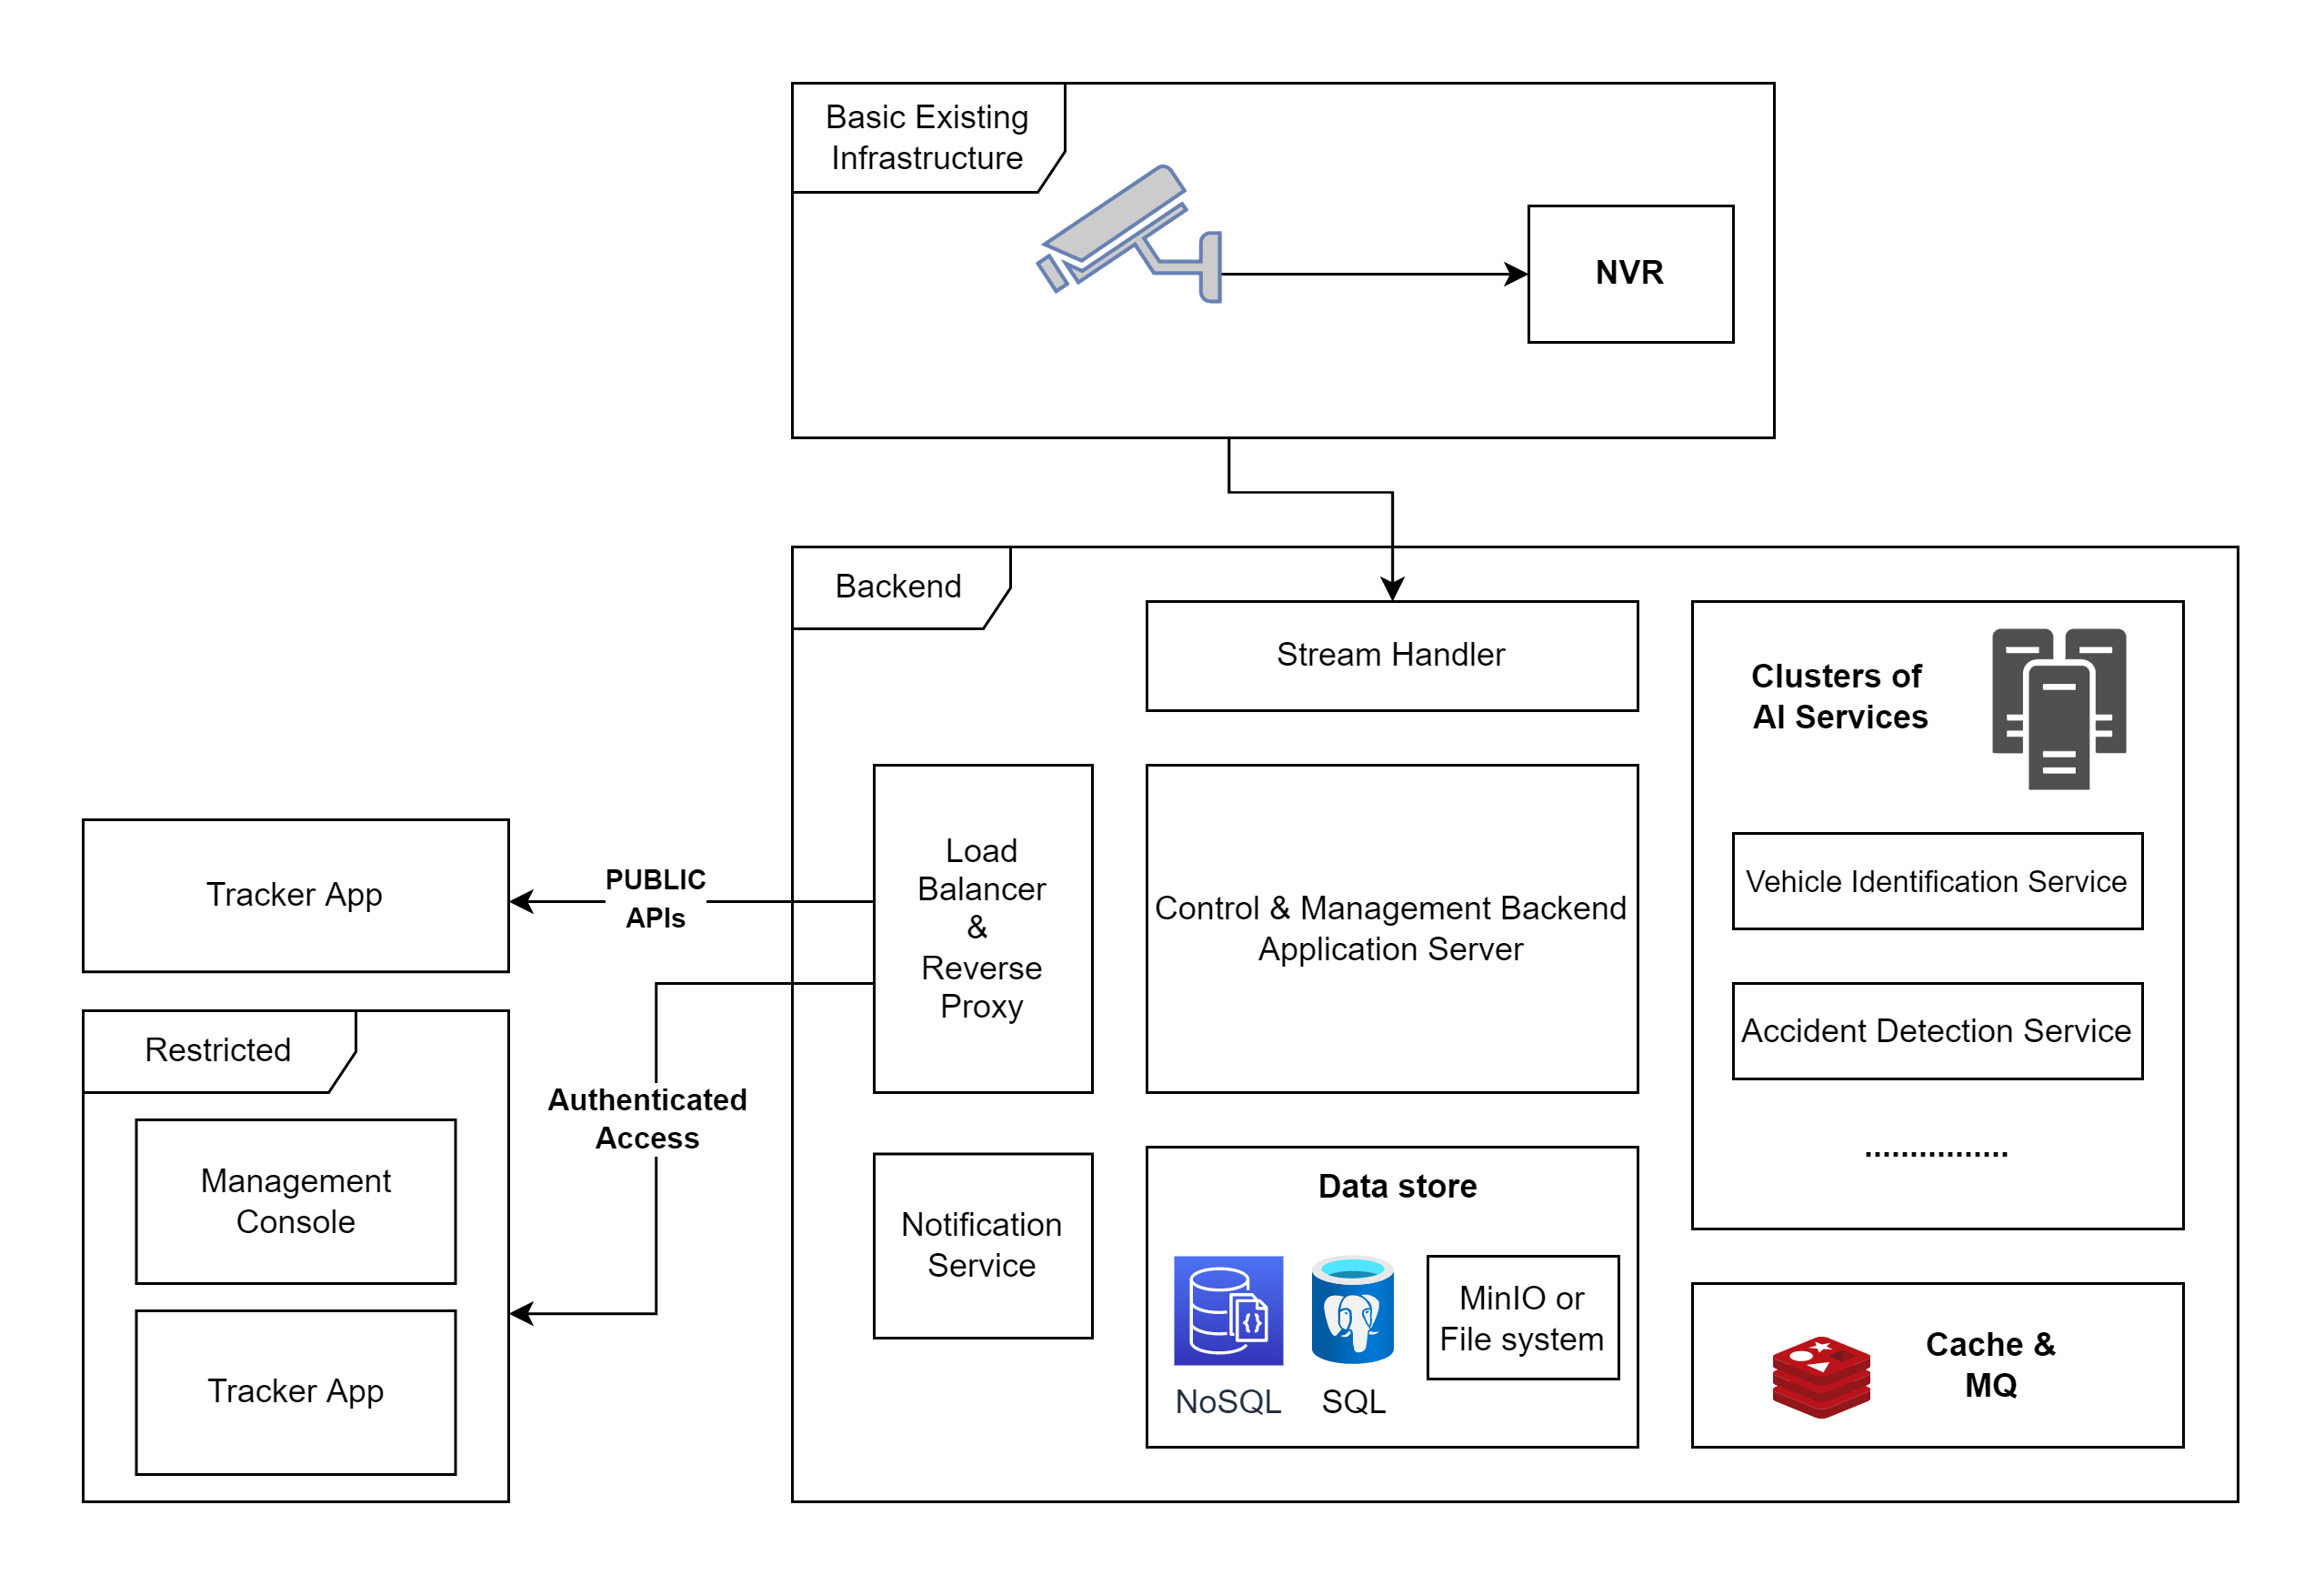
\includegraphics[width=0.8\linewidth]{Images/architecture_high_level}
	\caption{High level system architecture}
	\label{fig:architecturehighlevel}
\end{figure}

\lipsum[1-2]

\begin{figure}
	\centering
	\begin{subfigure}[b]{0.8\linewidth}
		\centering
		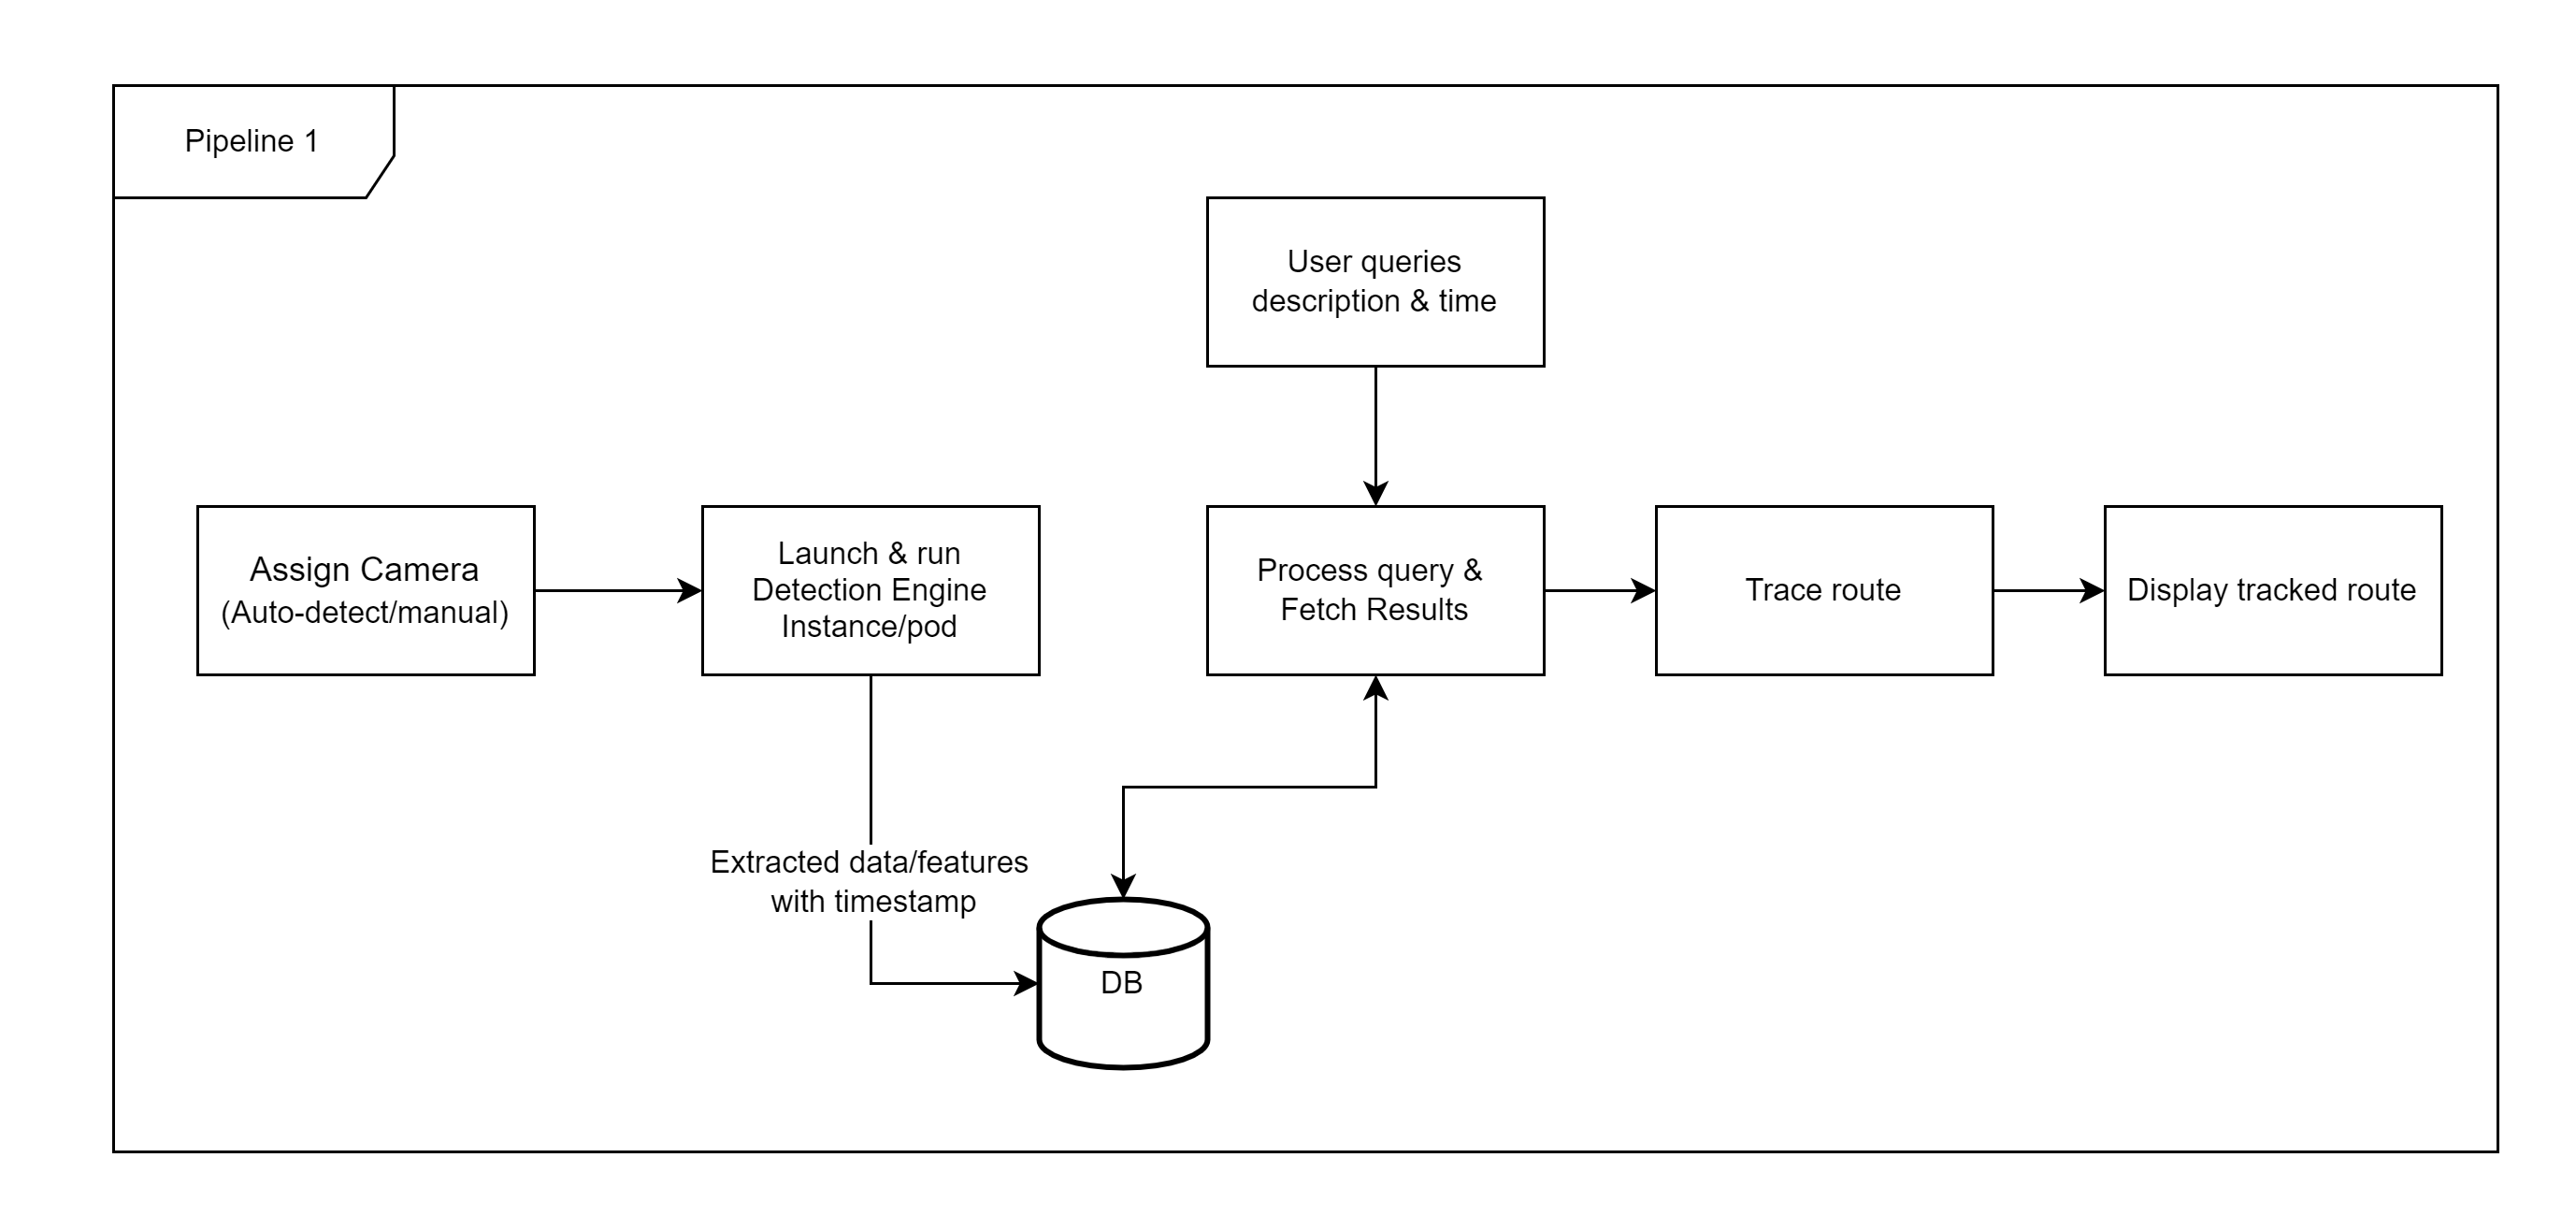
\includegraphics[width=\linewidth]{Images/pipeline1}
		\caption{pipeline1}
		\label{fig:pipeline1}
	\end{subfigure}

	\begin{subfigure}[b]{0.8\linewidth}
		\centering
		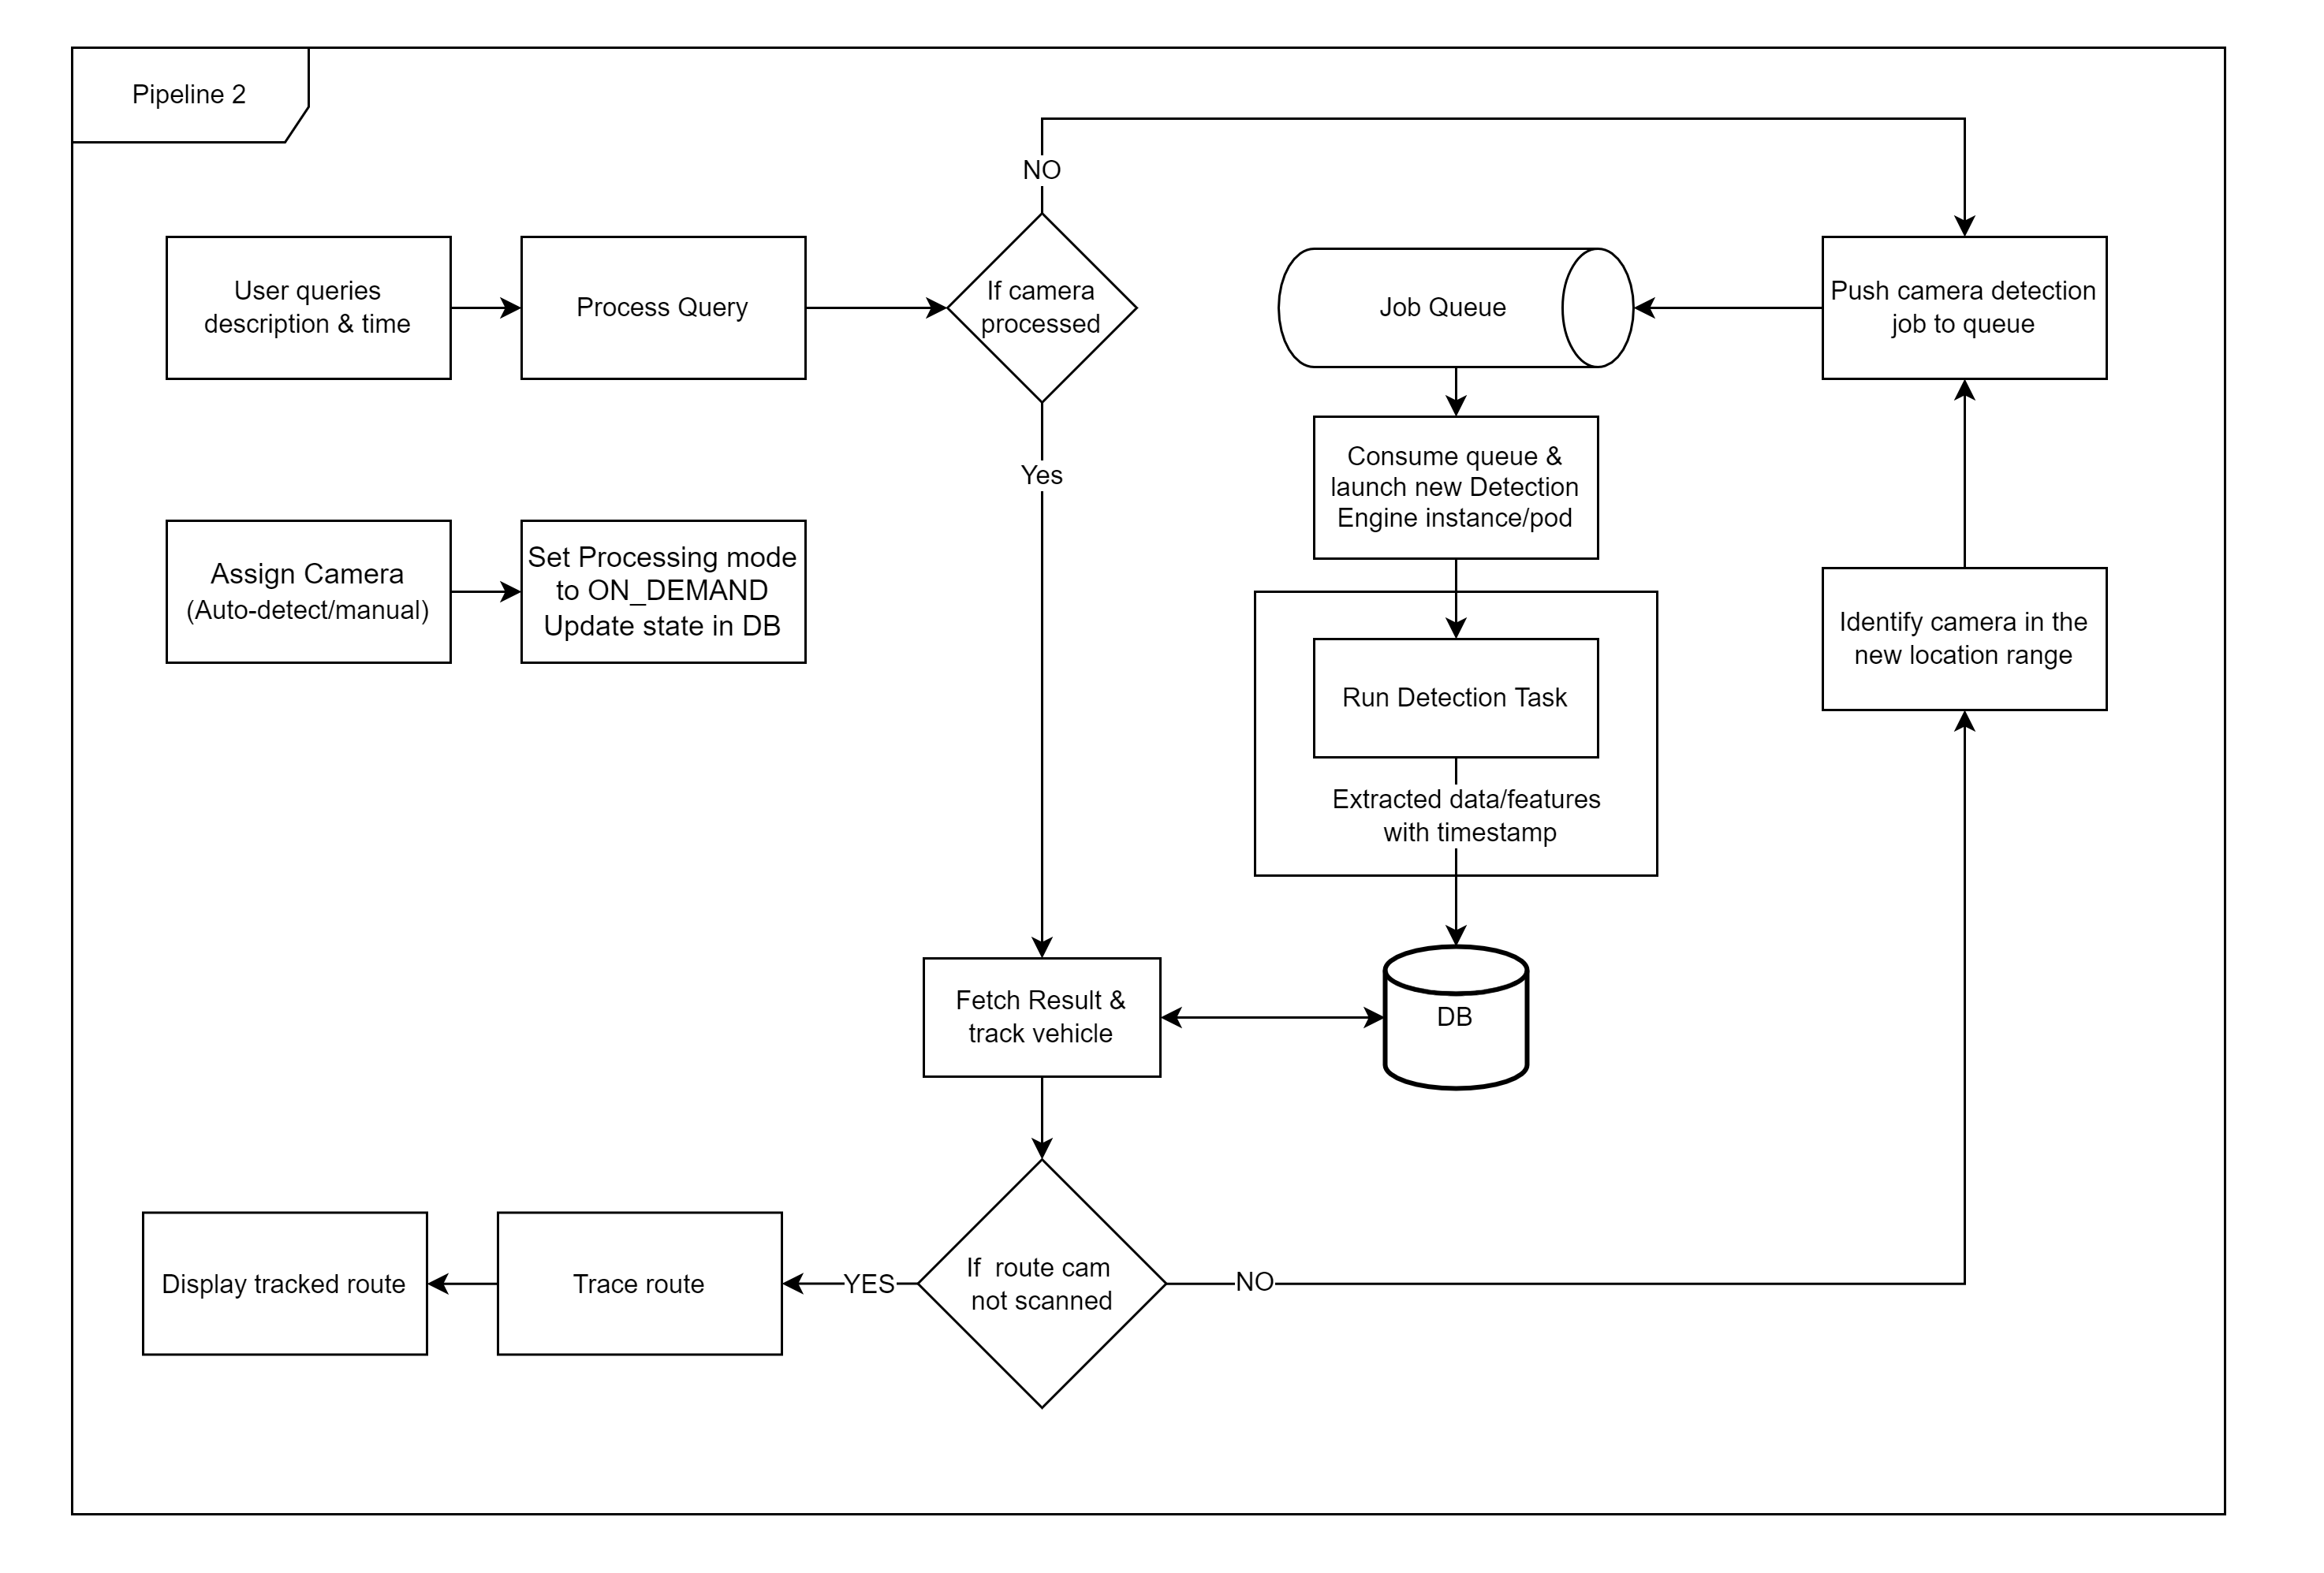
\includegraphics[width=\linewidth]{Images/pipeline2}
		\caption{pipeline2}
		\label{fig:pipeline2}
	\end{subfigure}
	\caption{Workflow pipeline}
\end{figure}

\lipsum[1-2]
 


\section{Camera Network}
The camera feed is obtained from a project deployed by Center for Information, Communication and Educational Technology (CICET), Government College of Engineering Kannur. Under the project entitled "Third eye", a virtual network was established covering an area of 350 $KM^2$, connecting 9 institutes. Using the existing cable network, various camera at installed allowing easy and secure storage and streaming. Currently the project houses holds about 190 cameras. Excess to these footage if obtained by secured virtual private junction.

\begin{figure}[!ht]
	\centering
	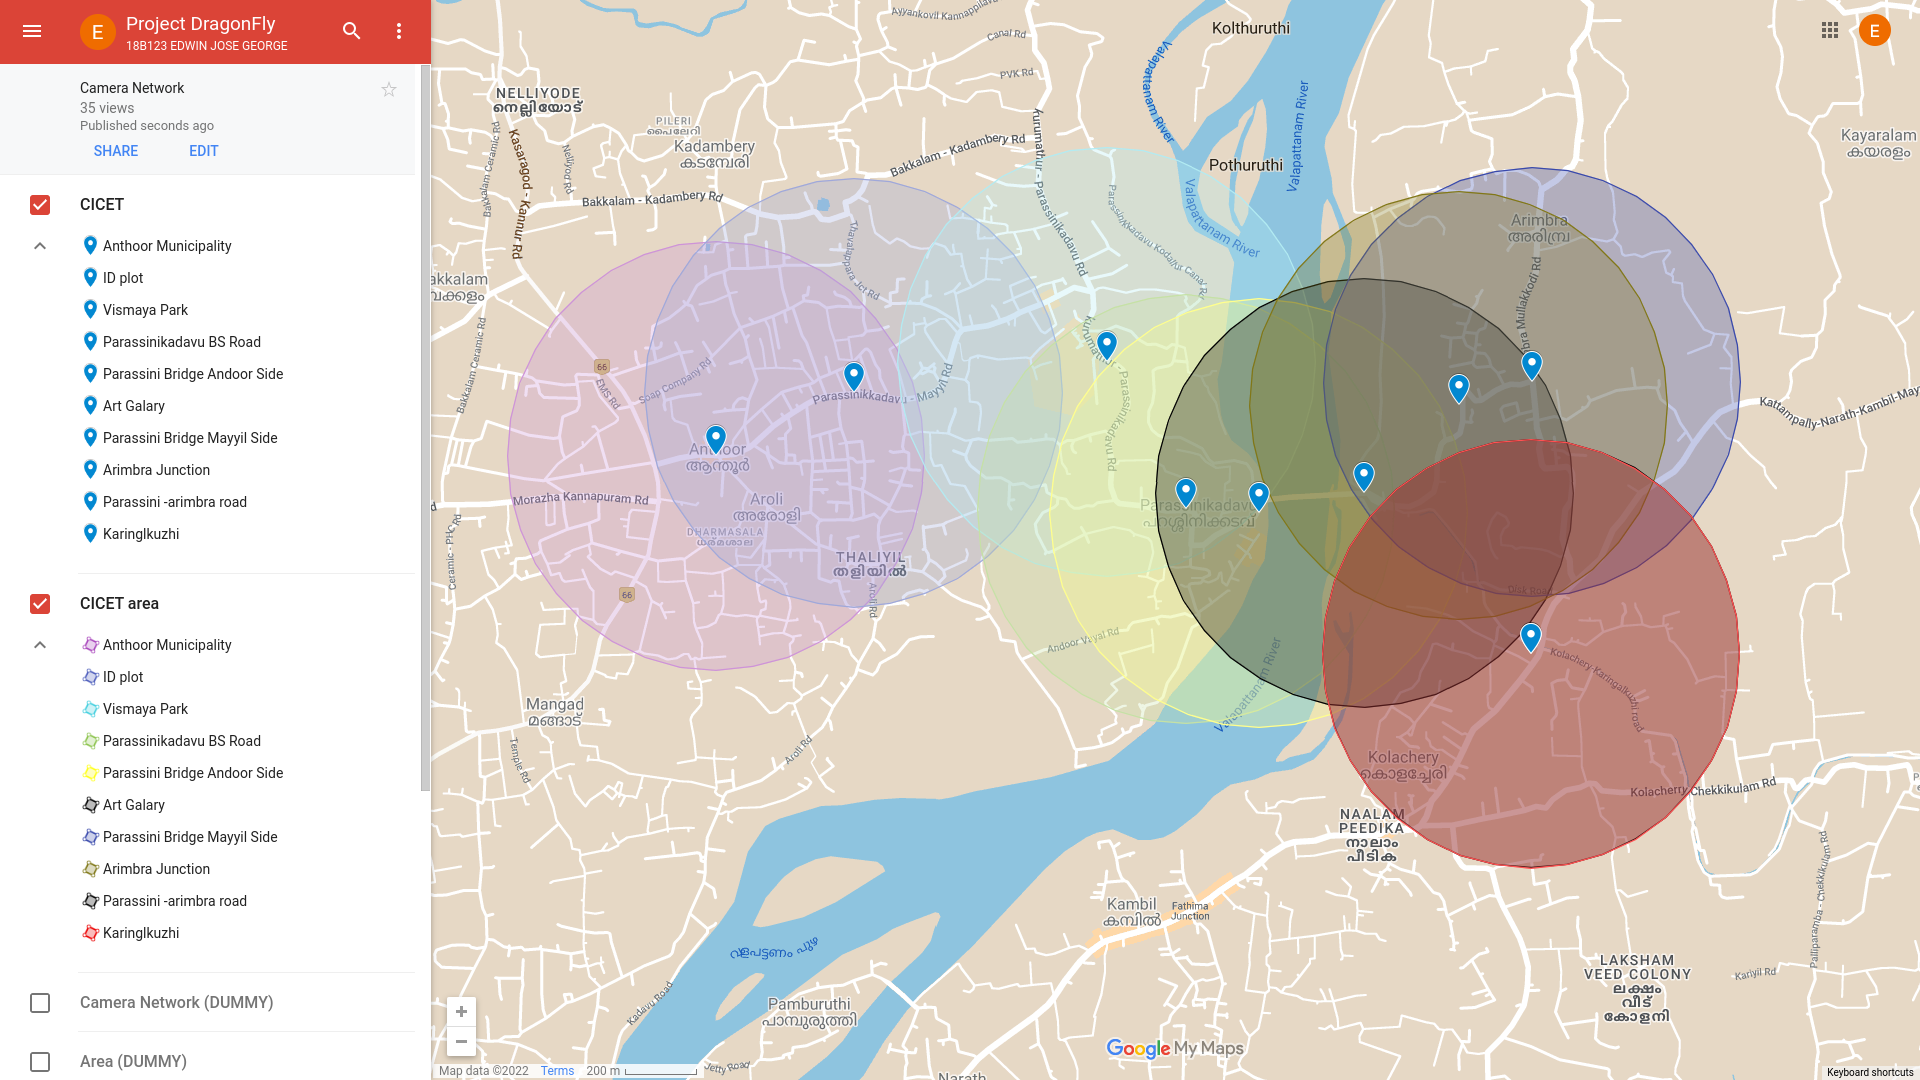
\includegraphics[width=\linewidth]{Images/camera-network}
	\caption{CICET camera network}
	\label{fig:camera-network}
\end{figure}

\begin{figure}[!ht]
	\centering
	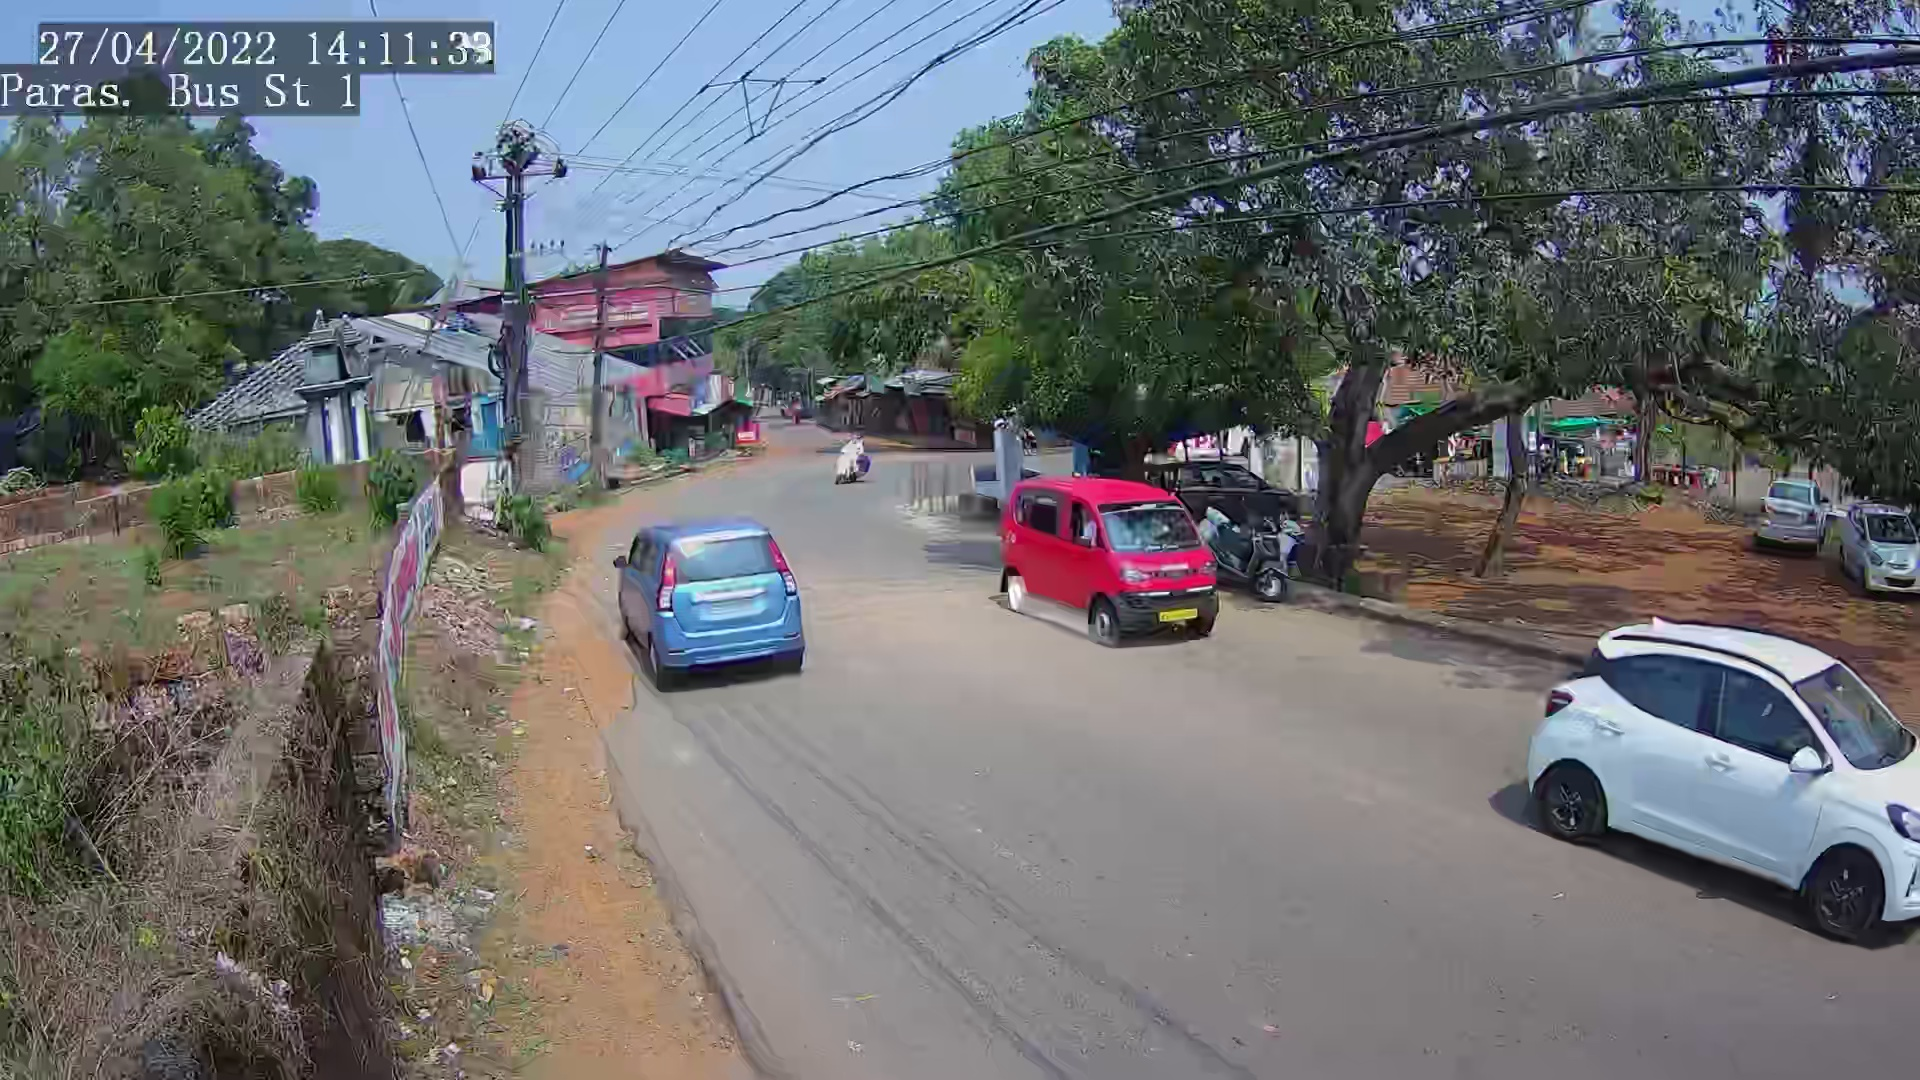
\includegraphics[width=0.32\linewidth]{Images/camera_footage/footage1} \hfill
	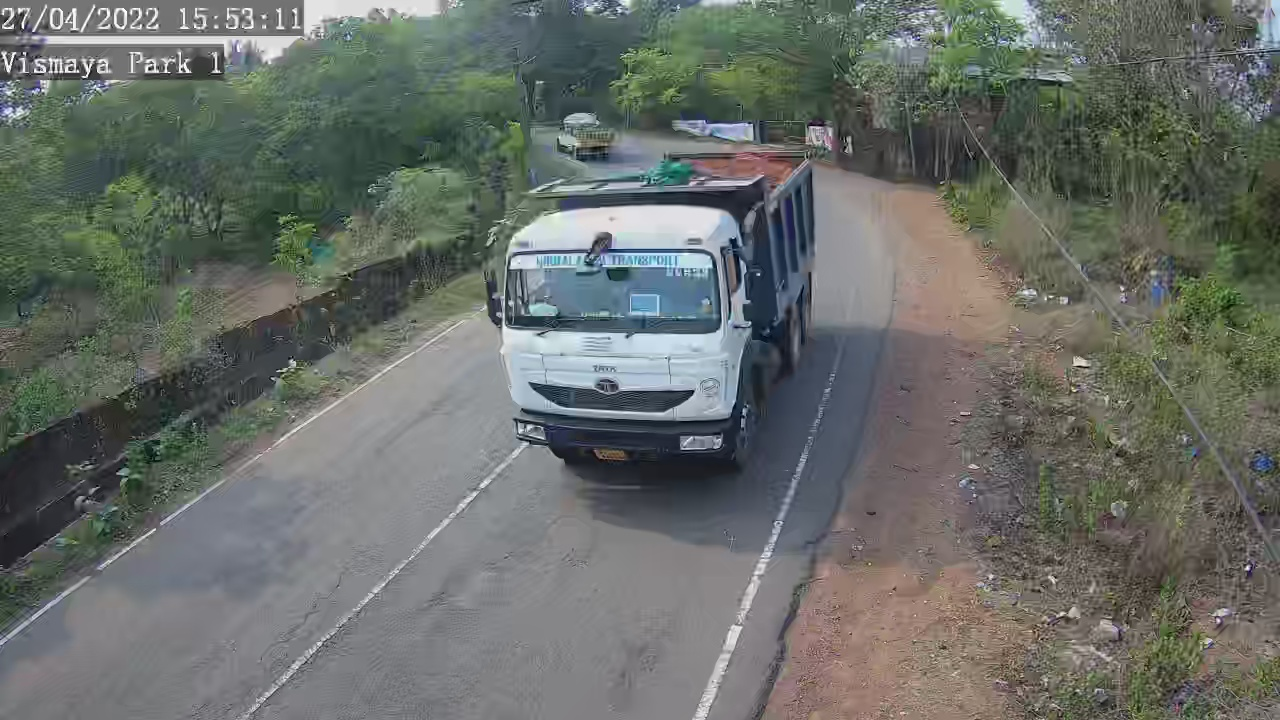
\includegraphics[width=0.32\linewidth]{Images/camera_footage/footage2} \hfill
%	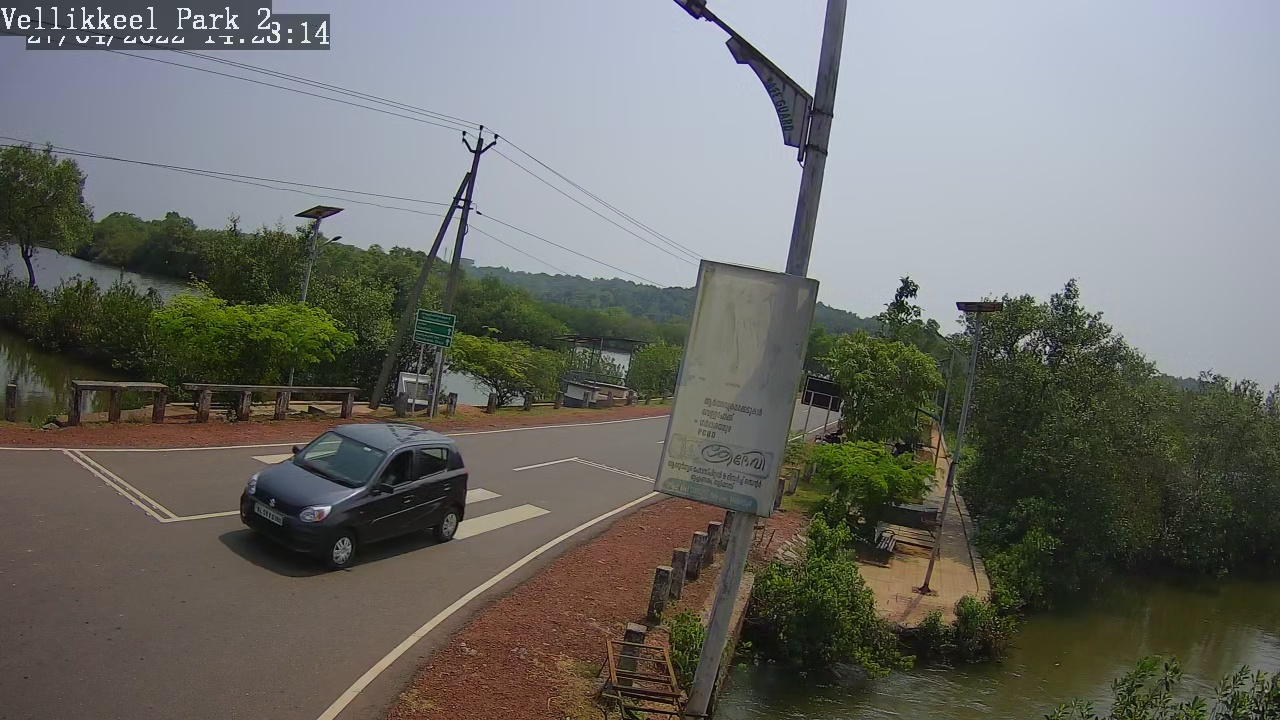
\includegraphics[width=0.32\linewidth]{Images/camera_footage/footage3} \\
%	\vspace{3mm}
%	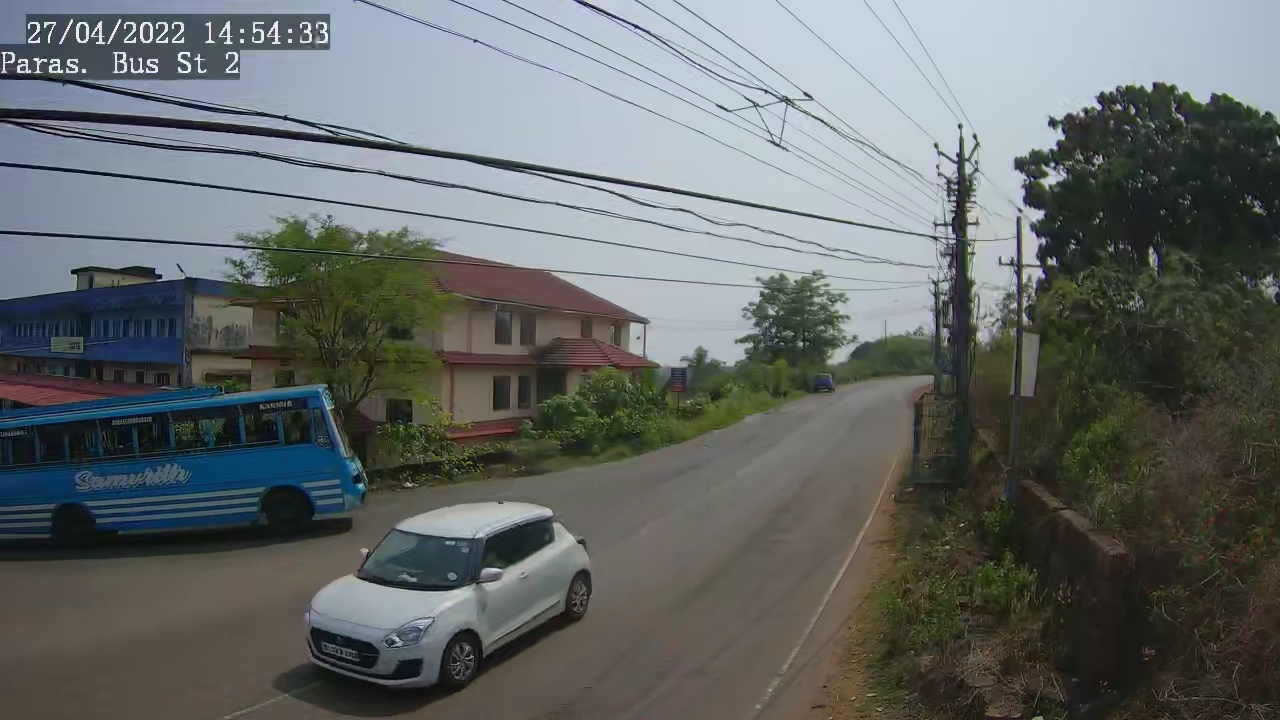
\includegraphics[width=0.32\linewidth]{Images/camera_footage/footage4} \hfill
	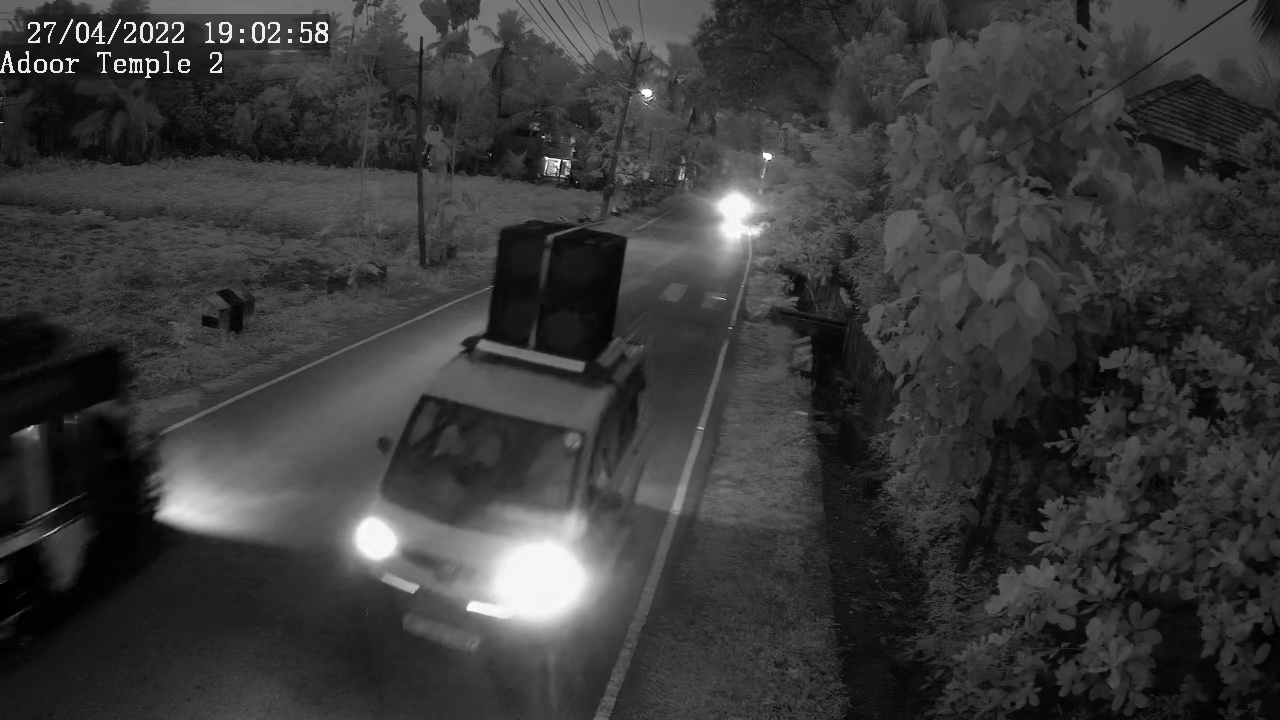
\includegraphics[width=0.32\linewidth]{Images/camera_footage/night1} \hfill
%	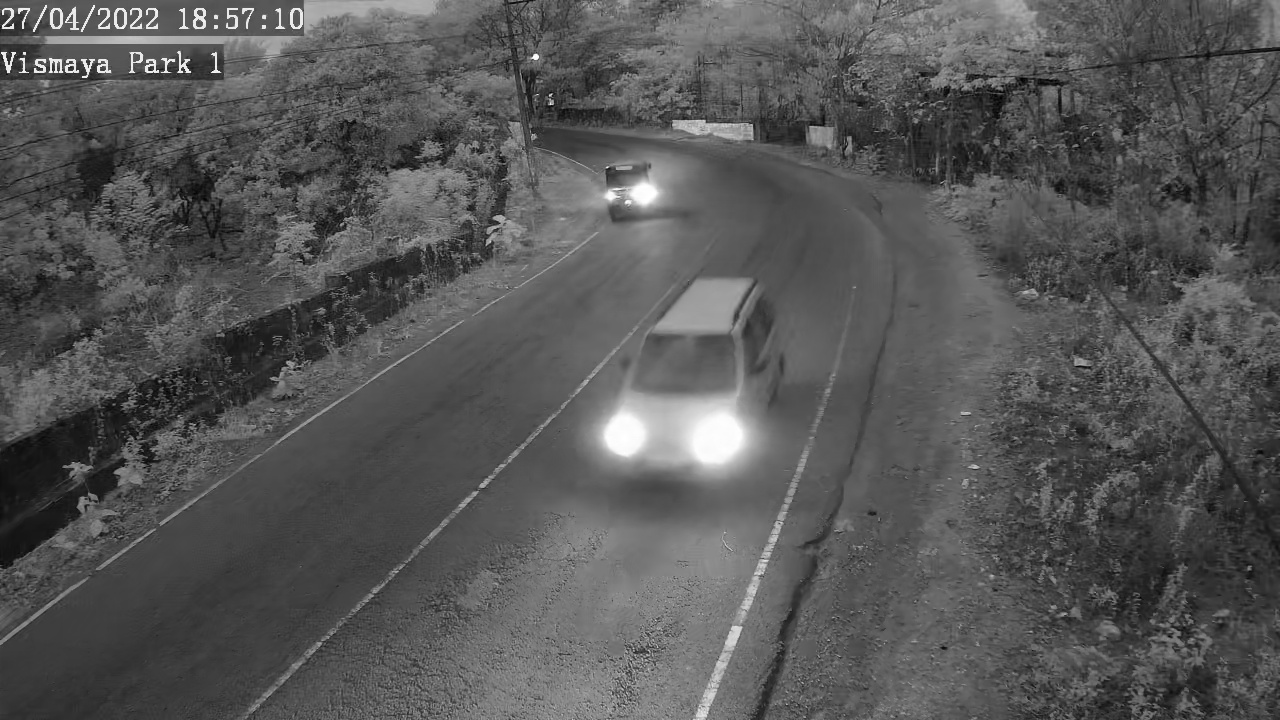
\includegraphics[width=0.32\linewidth]{Images/camera_footage/night2}
	\caption{Sample camera footage}
\end{figure}


\section{UI Design}

\lipsum[1]

\begin{figure}[!ht]
	\centering
	\begin{subfigure}[b]{0.48\linewidth}
		\centering
		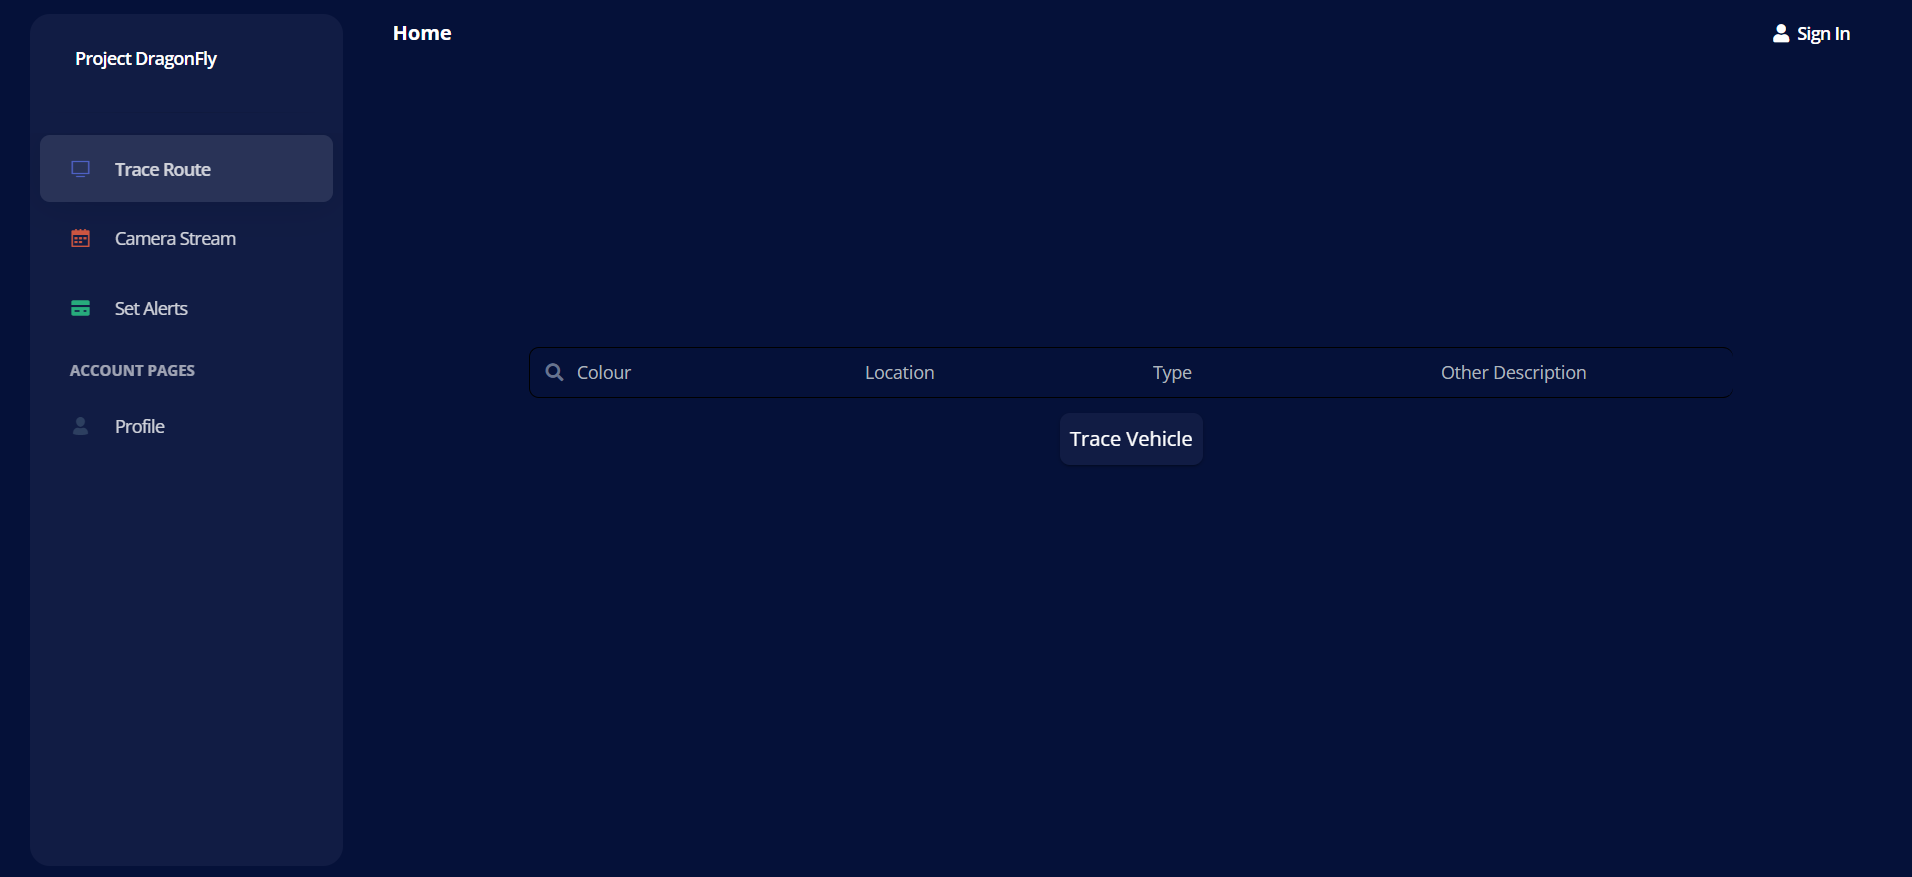
\includegraphics[width=\linewidth]{Images/UI/home}
		\caption{Home page}
		\label{fig:home}
	\end{subfigure} \hfill
	\begin{subfigure}[b]{0.48\linewidth}
		\centering
		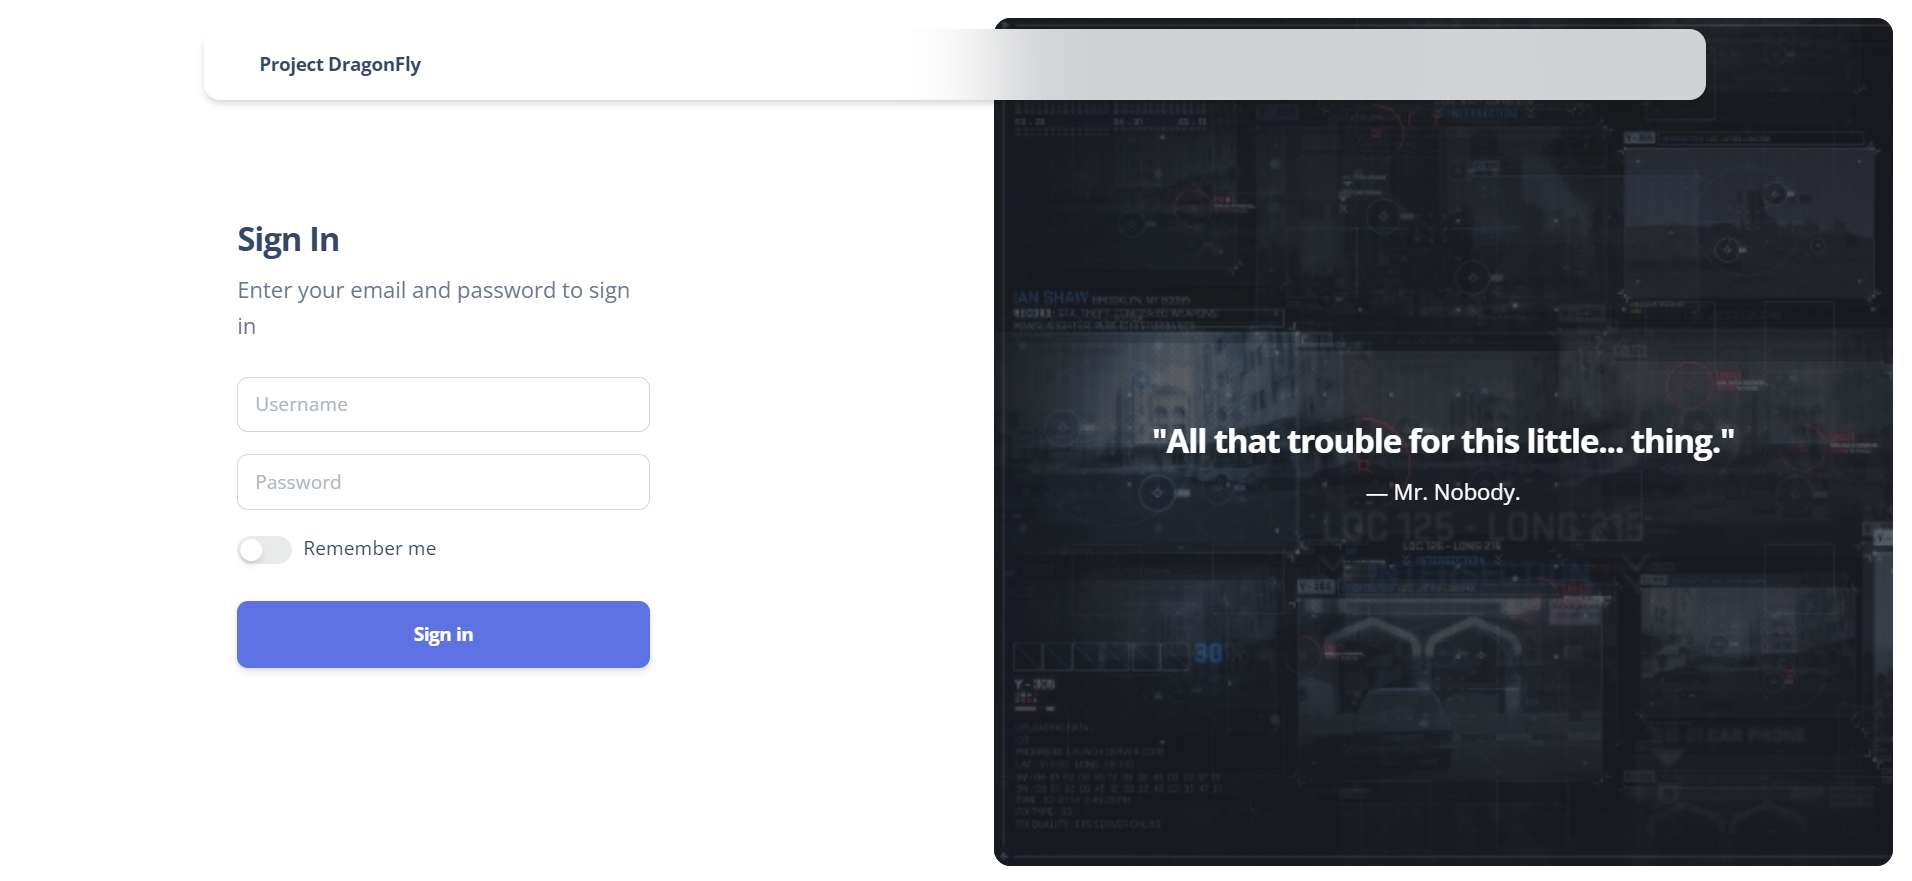
\includegraphics[width=\linewidth]{Images/UI/login}
		\caption{Login page}
		\label{fig:login}
	\end{subfigure} \\ \vspace{3mm}
	\begin{subfigure}[b]{0.48\linewidth}
		\centering
		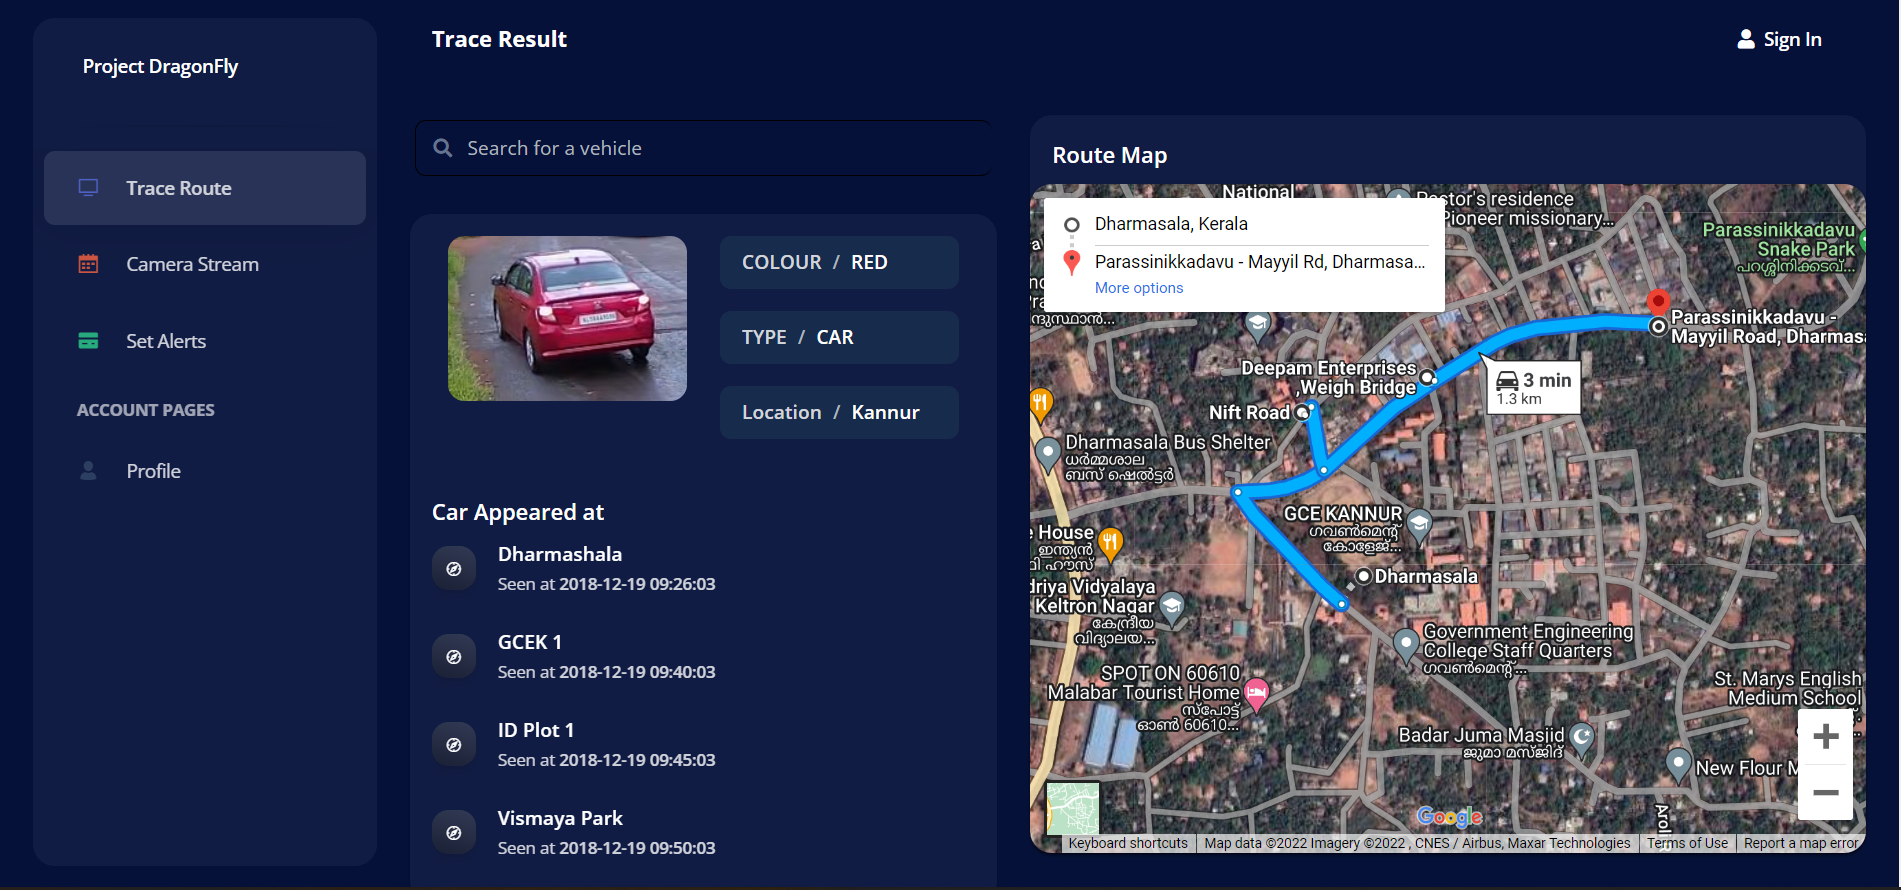
\includegraphics[width=\linewidth]{Images/UI/result}
		\caption{Result}
		\label{fig:result}
	\end{subfigure} \hfill
	\begin{subfigure}[b]{0.48\linewidth}
		\centering
		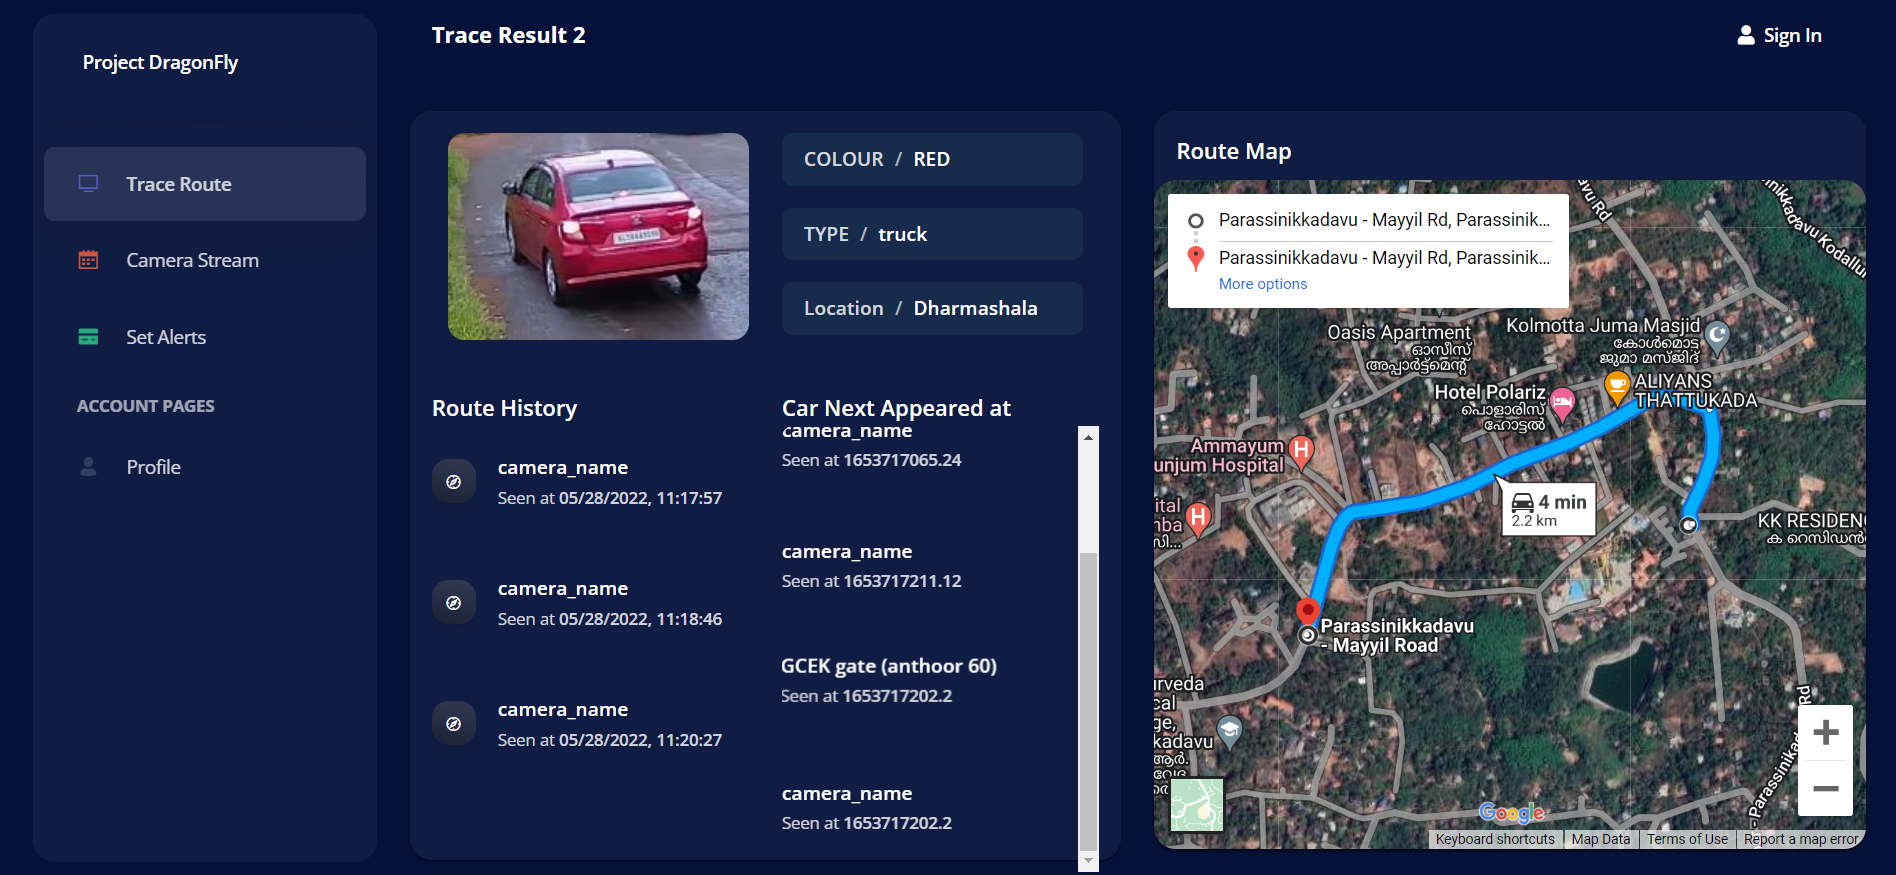
\includegraphics[width=\linewidth]{Images/UI/tracing}
		\caption{Tracing}
		\label{fig:tracing}
	\end{subfigure}
	\caption{UI Design}
\end{figure}

\lipsum[1]

\section{AI Model}
\lipsum[1-3]
\subsection{Image Dictionary}
\lipsum[1-2]

\section{Algorithm}
\lipsum[1-3]